\section{Data and Quality Control}
\label{sec:data}

\subsection{Network and acquisition}
We assembled hourly observations for the seven criteria pollutants---PM\textsubscript{2.5},
PM\textsubscript{10}, NO, NO\textsubscript{2}, SO\textsubscript{2}, CO and
O\textsubscript{3}---from $204$ continuous ambient monitoring stations across urban
India for calendar year 2025, retrieved through the OpenAQ v3 API \citep{openaq},
which aggregates and standardizes the regulatory CAAQMS/CPCB feeds. Each station was
merged, at hourly resolution, with collocated Open-Meteo reanalysis meteorology
\citep{openmeteo}: 2\,m air temperature, relative humidity, 10\,m wind speed, and
surface pressure, sampled at the nearest $\sim$0.1$^{\circ}$ reanalysis grid cell and
cached per coordinate to avoid redundant retrieval. All timestamps are stored in UTC;
because the network spans a single nominal time zone (Indian Standard Time, UTC+5:30),
diurnal features are computed after conversion to local solar-aligned hours. The
assembled corpus comprises $1{,}180{,}551$ station-hours.

\subsection{Coverage and completeness}
The realized corpus covers approximately $66\%$ of a complete
$204 \times 8{,}760$ station-hour grid (\cref{fig:coverage}a). Completeness is
markedly heterogeneous across sites: the median within-year coverage is $0.77$, but a
left tail of $37$ stations falls below $50\%$. Missingness is a mixture of structural
(no sensor deployed for a given species), intermittent (sensor dropout), and
below-detection values that are not separable in the absence of detection-limit
metadata. Per-species availability within present rows (\cref{fig:coverage}b) is high
for PM\textsubscript{2.5} ($0.98$) and the gases ($0.91$--$0.96$). Because
autocorrelated gaps interact dangerously with random splitting
(\cref{sec:methods}), all predictive evaluation uses blocked or grouped protocols
rather than imputing across gaps.

\begin{figure}[t]
  \centering
  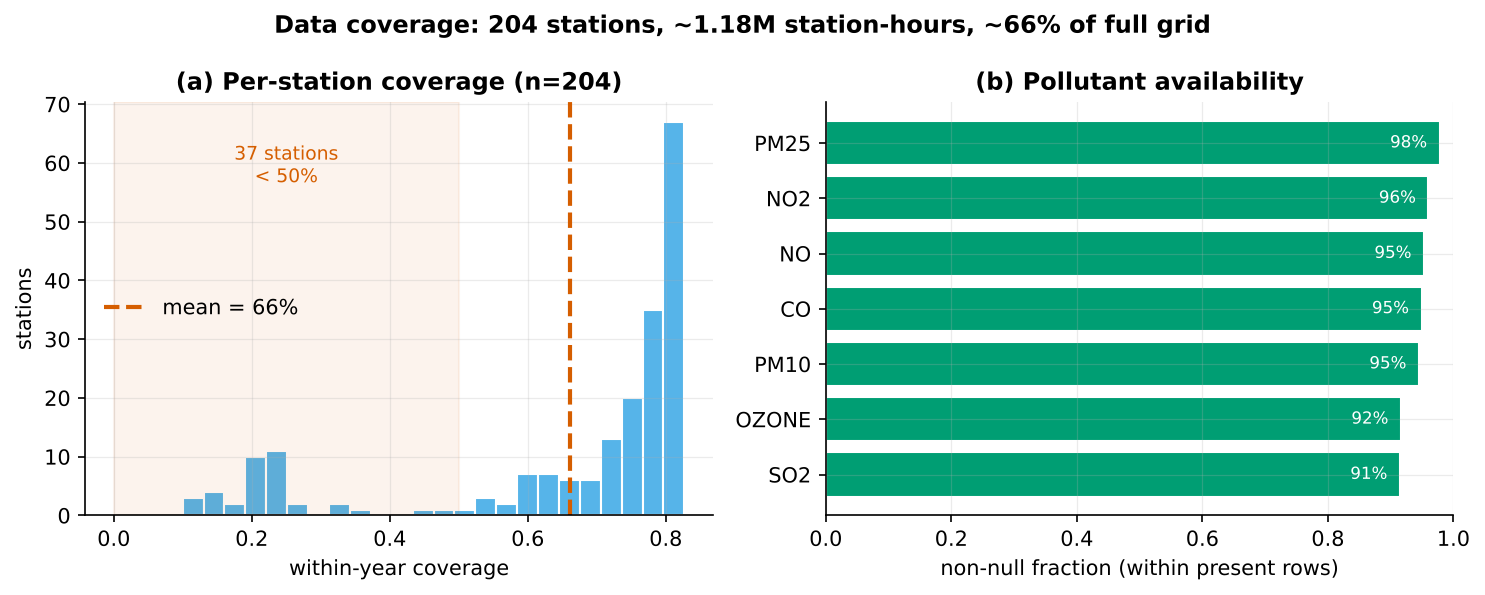
\includegraphics[width=0.98\linewidth]{fig1_network_coverage.png}
  \caption{Network coverage. (a) Distribution of within-year temporal completeness
  across the $204$ stations (mean $66\%$; $37$ stations below $50\%$, shaded).
  (b) Per-pollutant non-null fraction within present station-hours. Geolocation of
  individual monitors is not retained in the public telemetry export and is therefore
  not mapped; the network is urban and spatially concentrated in the National Capital
  Region and major metropolitan centres (a representativeness limitation, \cref{sec:gate}).}
  \label{fig:coverage}
\end{figure}

\subsection{Sanitization}
Three classes of non-physical artifact were identified and flagged. (i) \emph{Instrument
saturation / round caps}: distinct spikes of mass at round ceilings
(NO, NO\textsubscript{2}, O\textsubscript{3} near $500$; PM\textsubscript{2.5} near
$1000$). (ii) \emph{Zero-padding and dropout}: runs of exact zeros and abrupt gaps
inconsistent with ambient variability. (iii) \emph{Non-physical outliers}: $35$ values
exceeding physically plausible bounds were flagged and excluded from distributional
summaries. Screening these artifacts materially changes downstream covariance
estimates---for example, the CO--NO correlation rises from $0.14$ to $0.42$---which is
itself evidence that naive clustering is sensitive to data hygiene (\cref{sec:results}).

\subsection{The unit-provenance discovery}
\label{sec:units}
A pre-registration-style verification of measurement units against the
\emph{authoritative} OpenAQ per-sensor metadata revealed a material provenance defect
(\cref{fig:units}). NO is reported in parts-per-billion (ppb) at every station;
O\textsubscript{3}, PM\textsubscript{2.5} and PM\textsubscript{10} are reported in
mass concentration (\ugm{}) and are unit-consistent. However, CO, NO\textsubscript{2}
and SO\textsubscript{2} carry \emph{duplicate sensors reporting in both ppb and \ugm{}}
at almost every station (CO at $183/198$ stations, NO\textsubscript{2} at $187/199$,
SO\textsubscript{2} at $178/191$), while the exported telemetry retains a single value
per pollutant per station-hour with \emph{no record of which sensor produced it}. A
mixing ratio (ppb) and a mass concentration (\ugm{}) are related only through molecular
weight and ambient temperature and pressure; they are not comparable, and the mix
cannot be reconciled post hoc from the stored data. This supersedes an earlier,
value-based inference (which had suggested a uniform CO regime): the authoritative
sensor metadata governs. Consequently, we restrict all quantitative cross-station
inference to the unit-consistent species (NO, O\textsubscript{3},
PM\textsubscript{2.5}, PM\textsubscript{10}); the two headline results below---ozone
estimation and the NO$\rightarrow$O\textsubscript{3} association---depend only on these.

\begin{figure}[t]
  \centering
  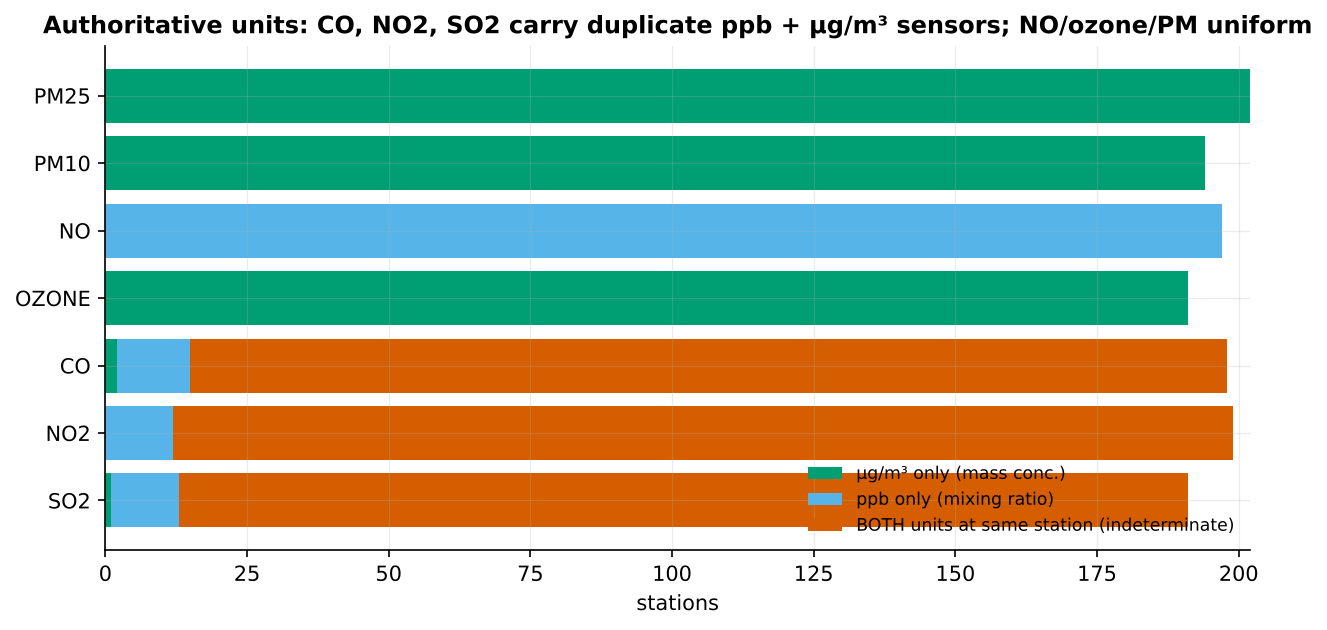
\includegraphics[width=0.92\linewidth]{fig6_units_verification.png}
  \caption{Authoritative unit verification per species. PM\textsubscript{2.5},
  PM\textsubscript{10} and O\textsubscript{3} are uniform \ugm{}; NO is uniform ppb;
  CO, NO\textsubscript{2} and SO\textsubscript{2} carry duplicate ppb and \ugm{}
  sensors at the same station (orange), rendering their stored unit indeterminate.}
  \label{fig:units}
\end{figure}

\subsection{Summary statistics}
\cref{tab:summary} reports distributional summaries of the sanitized telemetry.
Values are in the stored measurement scale; for the unit-indeterminate species
(CO, NO\textsubscript{2}, SO\textsubscript{2}) the magnitudes are not cross-station
comparable and are shown for completeness only. The heavy right skew of
PM\textsubscript{2.5} and PM\textsubscript{10} (large standard deviations, high 95th
percentiles) is characteristic of the Indian urban winter particulate regime.

\begin{table}[t]
  \centering
  \caption{Summary statistics of the sanitized telemetry (calendar year 2025,
  $204$ stations). Missing fraction is relative to present station-hours.
  CO, NO\textsubscript{2}, SO\textsubscript{2} are unit-indeterminate
  (\cref{sec:units}); PM in \ugm{}, O\textsubscript{3} in \ugm{}, NO in ppb.}
  \label{tab:summary}
  \begin{tabular}{lrrrrr}
    \toprule
    Pollutant & Mean & Std.\ dev. & 5th pct. & 95th pct. & Missing frac. \\
    \midrule
    O\textsubscript{3}            & 30.52  & 30.89  & 2.57  & 89.80  & 0.084 \\
    NO                            & 14.81  & 29.13  & 0.88  & 49.20  & 0.047 \\
    NO\textsubscript{2}           & 27.33  & 27.37  & 2.60  & 80.10  & 0.040 \\
    CO                            & 0.87   & 2.40   & 0.10  & 2.18   & 0.051 \\
    SO\textsubscript{2}           & 13.47  & 25.67  & 1.75  & 35.20  & 0.085 \\
    PM\textsubscript{10}          & 121.50 & 116.48 & 18.20 & 349.20 & 0.055 \\
    PM\textsubscript{2.5}         & 58.28  & 73.79  & 6.50  & 185.00 & 0.022 \\
    \bottomrule
  \end{tabular}
\end{table}
